\chapter{GIT HISTORY}

To ensure proper version control and systematic project management, the Medora Hospital Management System has been maintained using Git and hosted on GitHub. This enables efficient tracking of code updates, bug fixes, feature enhancements, and module developments over time.By using Git, every modification made to the system—including updates to modules such as Admin, Reception, Doctor, Pharmacy, Laboratory, and Billing—is recorded with commit history. This makes it easier to monitor progress, manage collaborative development, and revert to previous stable versions if necessary.The GitHub repository serves as a centralized platform for storing and managing the Laravel project structure, including folders such as app, bootstrap, config, database, public, resources, routes, and storage. It ensures that the latest version of the project is securely available for development, testing, and future deployment.

\begin{figure}[H]
    \centering
    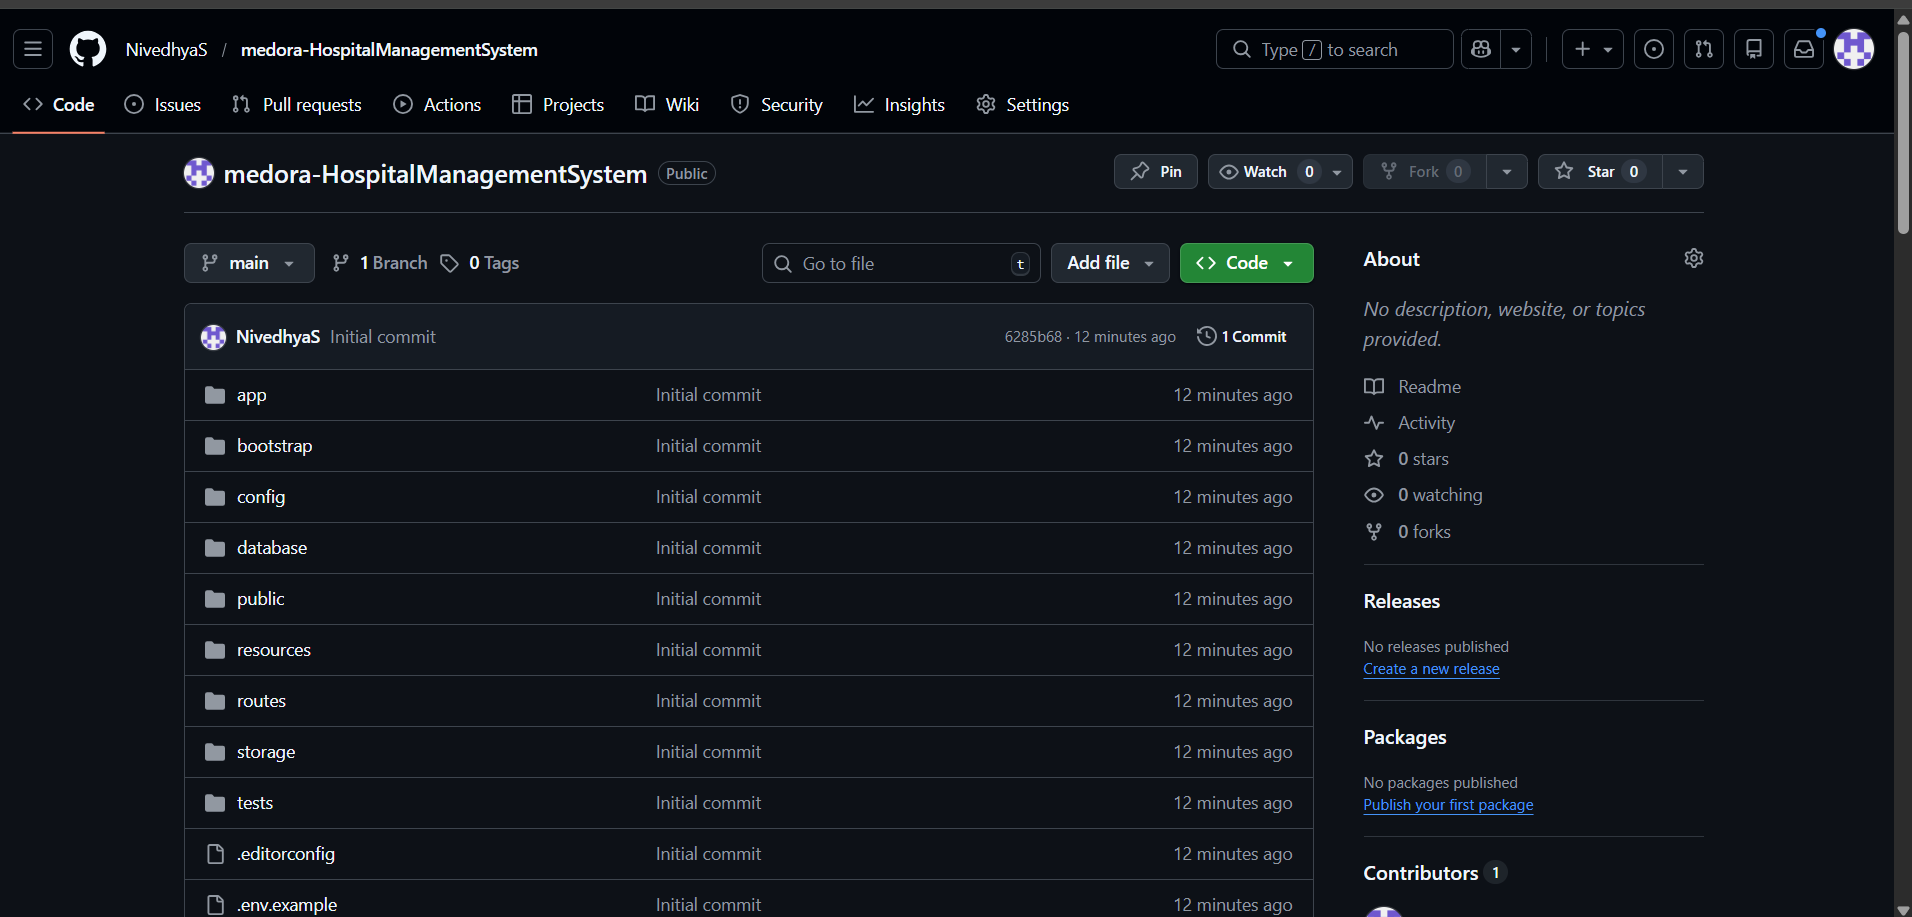
\includegraphics[width=1\textwidth]{git1.png}
    \caption{GitHub Repository – Initial Commit}
    \label{fig:git_repo}
\end{figure}

\begin{figure}[H]
    \centering
    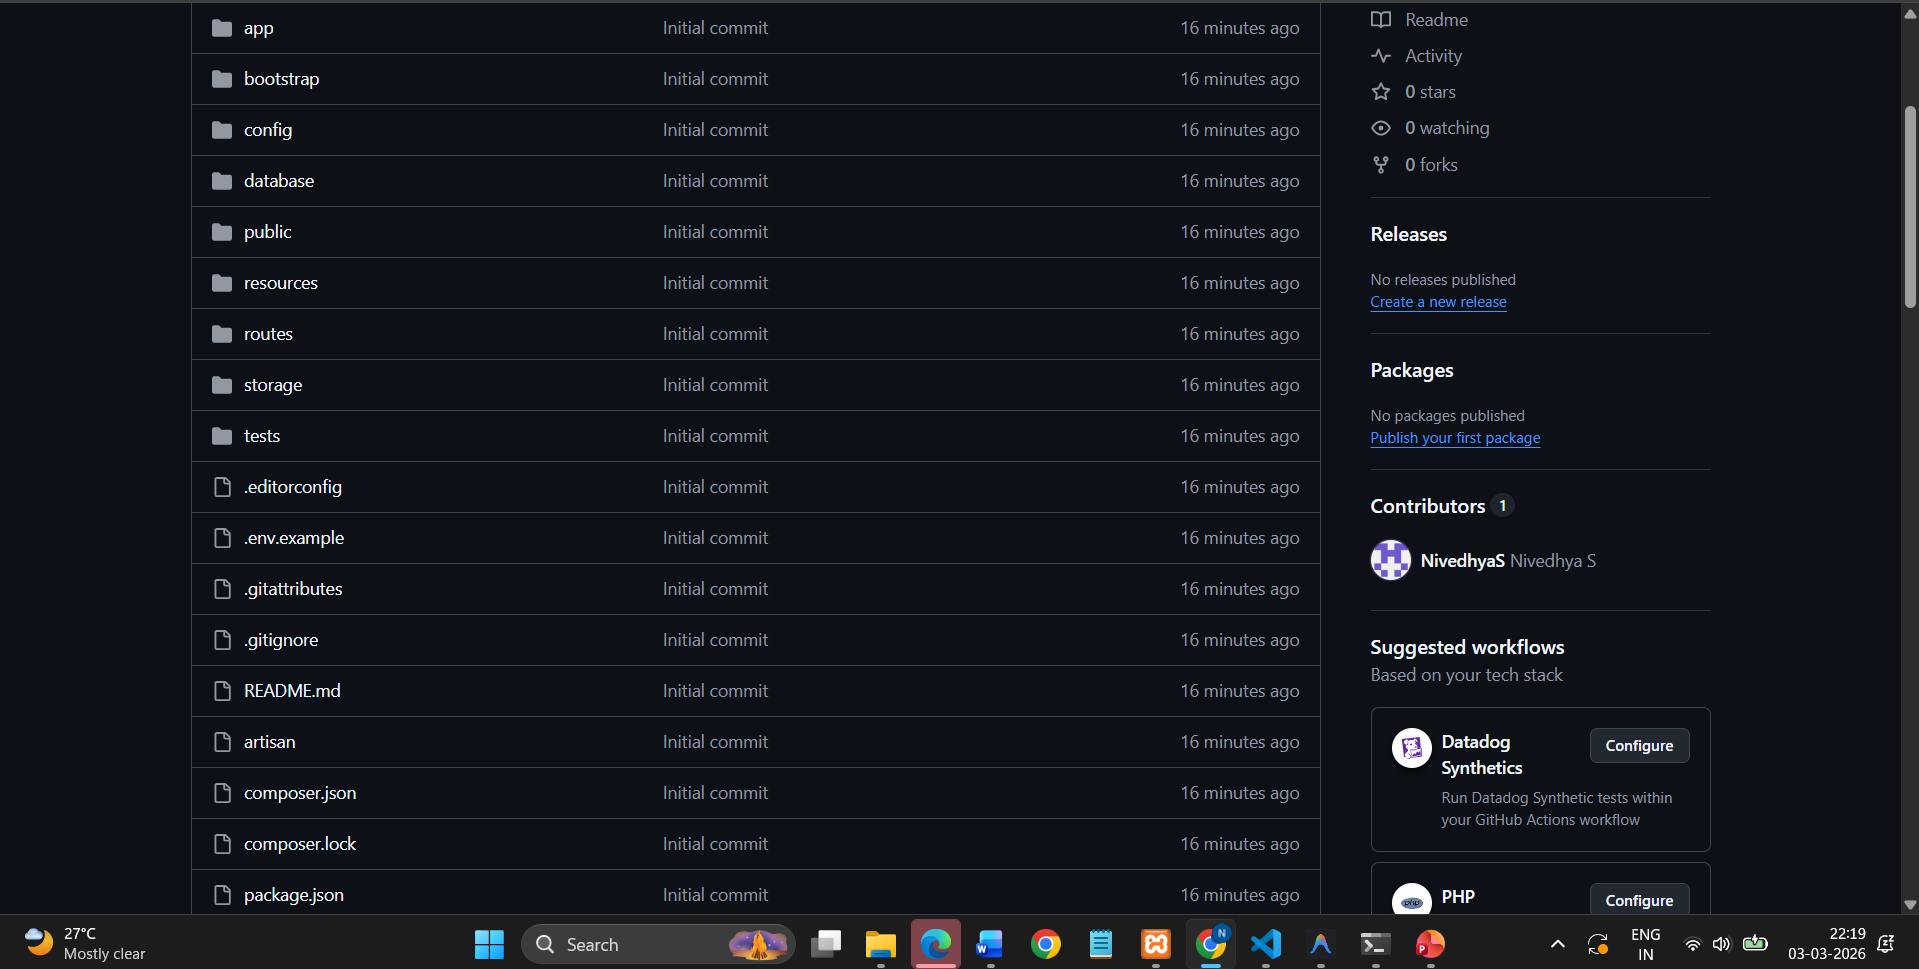
\includegraphics[width=1\textwidth]{git2.png}
    \caption{Project Directory Structure in GitHub}
    \label{fig:project_structure}
\end{figure}